\clearpage
\chapter{Blues, Pentatonic and Modal Writing}
\label{chap:blues-pentatonic-modal}

\classquote{音乐之所由来者远矣，生于度量，本于太一。}{L\"ushi Chunqiu, ``Great Music'' (《吕氏春秋·仲夏纪·大乐》)}{Translation: ``Music has deep origins; it is born of measure and rooted in the Great One.'' Pentatonic scales, the blues and church modes come from different traditions, yet each turns pitch measure into direct feeling.}

\section*{What you can do after this chapter}
\begin{itemize}
  \item Write major/minor pentatonic and blues scales, and explain why ``blue notes'' make the sound dirty but alive.
  \item Build a playable 12-bar blues progression and know where I--IV--V fall bar by bar.
  \item Identify the characteristic tone of Dorian, Lydian, Mixolydian and Phrygian, and choose a chord bed that does not fight it.
  \item In Yeban, lay a pentatonic/blues riff and an eight-bar modal vamp that stands without functional V--I.
\end{itemize}

\section{Pentatonic is not ``a major scale with two notes removed''}

Major pentatonic takes degrees 1, 2, 3, 5, 6; minor pentatonic takes 1, \(\flat\)3, 4, 5, \(\flat\)7. It removes the degrees most likely to create semitone clashes (4 and 7 in major; the neighbourhood of 2 and 6 in minor), so fast lines do not collide with the harmony. Its stability comes from two facts: adjacent notes are at least two semitones apart, and any ordering of the five notes stays free of sharp semitone adjacency.

But pentatonic is not only for folk tunes. Treat it as a usable pitch set, not a strict scale:

\begin{enumerate}
  \item \textbf{Melodic skeleton}: write the main phrase in pentatonic, then add 4 and 7 as passing tones.
  \item \textbf{Chord-tone filter}: if root, third and fifth all belong to the pentatonic set, the passage is more consonant.
  \item \textbf{Reharmonisation}: the same pentatonic melody can take different chords, as long as a chord third does not sit in long semitone conflict with the melody.
\end{enumerate}

\section{Blues scale and blue notes}

The minor blues scale is usually written:

\[
\mathrm{1\ \flat3\ 4\ \flat5\ 5\ \flat7\ 1}
\]

It inserts \(\flat\)5 into the minor pentatonic (1, \(\flat\)3, 4, 5, \(\flat\)7). That \(\flat\)5 is the classic ``blue note'': it is not a stable degree of major or minor, but a passing, ornamental or tension tone. The three common blue notes are \(\flat\)3, \(\flat\)5 and \(\flat\)7; they rub against the ``expected'' 3, 5, 7, and that rub is the blues' dirt and life.

\begin{figure}[htbp]
\centering
\begin{tikzpicture}[x=1.1cm,y=0.5cm,font=\scriptsize]
  \foreach \i/\n/\h in {0/C/0,1/E$\flat$/3,2/F/5,3/G$\flat$/6,4/G/7,5/B$\flat$/10,6/C/12} {
    \draw[gray] (\i,-0.4) -- (\i,\h);
    \node[above=2pt] at (\i,\h) {\n};
  }
  \draw[very thick] (0,0)--(1,3)--(2,5)--(3,6)--(4,7)--(5,10)--(6,12);
  \node[fill=white,inner sep=1.5pt] at (2.45,7.35) {\(\flat\)5 blue note};
\end{tikzpicture}
\caption*{Figure 10-1: C minor blues scale. \(\flat\)5 sits just before 5; it is the most visible tension point and belongs in passing, not as a long landing.}
\end{figure}

The blues scale can coexist with a major I7 chord: the chord is C7 (C E G B\(\flat\)), while the line may land on E\(\flat\) or G\(\flat\). This is not an error; blues treats the inside/outside conflict as colour. Two rules keep it usable:

\begin{itemize}
  \item Put blue notes on weak beats, short durations or passing positions; strong beats and phrase endings return to chord tones (root, 3, 5, \(\flat\)7).
  \item Do not make all three blue notes targets in one phrase; choose one signature note and use the others as ornament.
\end{itemize}

\section{Twelve-bar blues: skeleton and substitutions}

The basic twelve-bar blues, one bar per slot:

\[
\mathrm{I7\ I7\ I7\ I7\ \ IV7\ IV7\ I7\ I7\ \ V7\ IV7\ I7\ V7}
\]

I7, IV7 and V7 are all dominant-seventh in quality, not the triads of functional I--IV--V. Blues sevenths every chord so each has a seventh to resolve, which makes the sound more open. Common substitutions:

\begin{center}
\small
\begin{tabular}{cll}
\toprule
Bars & Basic & Common substitution \\
\midrule
9--12 & V7--IV7--I7--V7 & V7--IV7--I7--I7; or a turnaround VI7--V7 \\
5--8 & IV7--IV7--I7--I7 & IV7--IV7--I7--VI7 (set up the turnaround early) \\
Whole form & all dominant sevenths & replace some I7 with i7 or I6 to soften \\
\bottomrule
\end{tabular}
\end{center}

In Yeban: create 12 bars, place C7, F7 and G7 at the bar positions above; write the melody in C minor blues, landing C, E, G, B\(\flat\) on strong beats and putting E\(\flat\)/G\(\flat\) on weak beats. If it sounds too loose, remove \(\flat\)5 first and keep only \(\flat\)3 and \(\flat\)7.

\section{Modal writing: find the characteristic tone, then the chord bed}

The seven church modes are not seven scale names but seven ``tonic plus characteristic tone'' listening contracts. Ask first: which degree is the characteristic tone, and what interval does it make with the tonic?

\begin{center}
\small
\begin{tabular}{clll}
\toprule
Mode & Characteristic tone & Interval from tonic & Writing note \\
\midrule
Dorian & major sixth & bright minor & usually i--IV; avoid strong V7 \\
Lydian & augmented fourth & floating, less grounded & I--II; little V \\
Mixolydian & minor seventh & open, bluesy & I7--IV; V7 optional \\
Phrygian & minor second & tense, exotic & i--\(\flat\)II; avoid chains of minor seconds \\
Aeolian & minor sixth & natural-minor base & same shape as natural minor \\
Locrian & minor second + diminished fifth & very unstable & rarely tonic; use locally \\
Ionian & major seventh & major base & same as major \\
\bottomrule
\end{tabular}
\end{center}

The key difference from functional writing: functional harmony pins ``home'' with V--I; modal writing holds the centre with a \textbf{sustained tonic bed} and repeated \textbf{characteristic tone}. In a pure modal passage a strong V7 tends to pull the ear back to major/minor, so cycles such as i--IV, I--II or i--\(\flat\)VII are preferred because they do not resolve.

\begin{figure}[htbp]
\centering
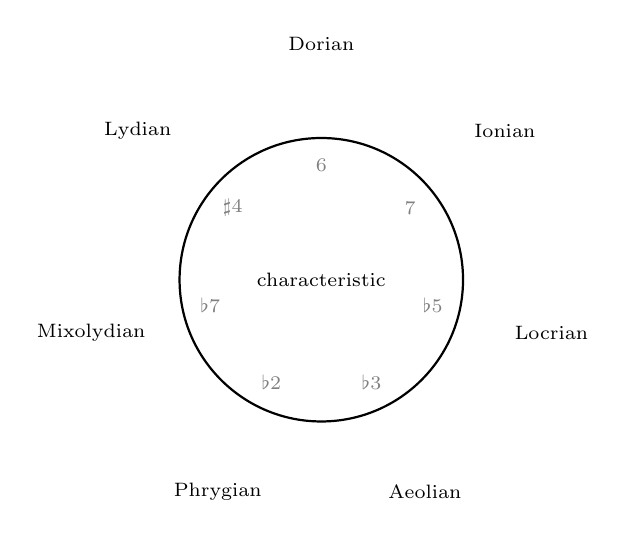
\begin{tikzpicture}[font=\scriptsize]
  \draw[->,thick] (0,0) circle (1.8);
  \foreach \a/\m/\t in {90/Dorian/6, 141/Lydian/\sharp4, 193/Mixolydian/\flat7, 244/Phrygian/\flat2, 296/Aeolian/\flat3, 347/Locrian/\flat5, 39/Ionian/7} {
    \node at (\a:3.0) {\m};
    \node[gray] at (\a:1.45) {$\t$};
  }
  \node at (0,0) {characteristic};
\end{tikzpicture}
\caption*{Figure 10-2: A mode's ID card is its characteristic tone. Learn which interval differs from the tonic, then choose the chord bed.}
\end{figure}

\section{Blues, pentatonic and modal writing in real songs}

\begin{itemize}
  \item \textbf{Chuck Berry, ``Johnny B. Goode''}: Anchors rock-and-roll guitar bends on the 12-bar I--IV--V blues frame, turning the tension between minor and major thirds into kinetic drive.
  \item \textbf{Jay Chou, ``Blue and White Porcelain'' (青花瓷)}: Shapes a spacious Chinese pentatonic melody over modern functional pop harmony, blending traditional phrasing with contemporary warmth.
  \item \textbf{Miles Davis, ``So What''}: Holds D Dorian (Dm7) for 16 bars and shifts up a semitone to E$\flat$ Dorian for the bridge, proving a modal vamp creates a complete mood without constant chord changes.
\end{itemize}

\section{Exercises}

\begin{exercise}
\begin{enumerate}
  \item Write the seven notes of A minor blues and mark the three blue notes.\\
  \emph{Answer:} A C D E\(\flat\) E G A; blue notes C, E\(\flat\), G.
  \item In C blues, why can C7's E and the melody's E\(\flat\) coexist?\\
  \emph{Answer:} E\(\flat\) is a blue/passing tone and E is the chord third; the conflict is blues colour, controlled by metric position and duration, not by parking E\(\flat\) on a strong beat.
  \item Write a four-bar Dorian vamp using only i and IV, with no V7.\\
  \emph{Sample:} Dm7--G--Dm7--G; G is IV in D Dorian, and the characteristic B (major sixth) can be heard against Dm7.
  \item Harmonise the C major pentatonic line C--D--E--G--A with C, F and G in two orders; say which is smoother.\\
  \emph{Answer:} C--F--G keeps A farther from F; moving G earlier increases semitone friction around A.
  \item Why avoid a strong V7 in a modal passage?\\
  \emph{Answer:} Its leading tone pulls the centre back into major/minor functional harmony and breaks the floating centre held by the tonic bed.
  \item Build 12 bars in Yeban: bars 1--4 C7, 5--6 F7, 7--8 C7, 9--12 G7--F7--C7--G7; write two phrases in C blues and mark where the blue notes fall.\\
  \emph{Sample:} phrase 1 over four bars puts E\(\flat\) on weak beat 2 and G\(\flat\) as a passing note on beat 3; phrase 2 lands on G (the chord fifth), never parking a blue note on a strong beat.
\end{enumerate}
\end{exercise}

\section{Help topic mapping}
\begin{center}
\footnotesize
\setlength{\tabcolsep}{3pt}
\begin{longtable}{p{0.34\linewidth}p{0.45\linewidth}p{0.15\linewidth}}
\toprule
Section & In-app help anchor & Note \\
\midrule
\endhead
Pentatonic and blues scales & \texttt{music-theory-blues-scale} & Figure 10-1 \\
Twelve-bar blues & \texttt{music-theory-12-bar-blues} & Table 10-1 \\
Modal characteristic tones & \texttt{music-theory-modal-character} & Table 10-2 \\
Modal chord beds & \texttt{music-theory-modal-vamp} & Figure 10-2 \\
How to do it in Yeban & \texttt{music-theory-blues-riff} & Operation \\
Exercises & \texttt{music-theory-ch10-practice} & Answers in this chapter \\
\bottomrule
\end{longtable}
\end{center}

\section*{Further reading}
\addcontentsline{toc}{section}{Further reading}
\begin{itemize}
  \item \textbf{Wikipedia: Pentatonic scale}: \url{https://en.wikipedia.org/wiki/Pentatonic_scale}. Expands on pentatonic structures across global musical traditions.
  \item \textbf{Wikipedia: Twelve-bar blues}: \url{https://en.wikipedia.org/wiki/Twelve-bar_blues}. Covers classic twelve-bar blues chord variations and turnarounds.
  \item \textbf{Wikipedia: Mode (music)}: \url{https://en.wikipedia.org/wiki/Mode_(music)}. Compares the characteristic scale degrees and harmonic colour of the seven diatonic modes.
\end{itemize}
